%!TEX root =../MemoriaTFM.tex
%El anterior comando permite compilar este documento llamando al documento raíz
\chapter{Desarrollo de la solución}\label{chp-04}
\epigraph{As an engineer, you learn there is a solution to every problem. It may take you a while, but eventually you're going to find it.}{Tony Cárdenas\\American politician}

\lettrine[lraise=-0.1, lines=2, loversize=0.2]{E}{l} apartado actual está dedicado a comprender el proceso seguido durante el desarrollo de la solución realizada. Comenzando con una introducción que sitúe al lector en condiciones que le permitan reproducir el proceso presentado y los primeros pasos a seguir en la preparación del entorno, desplegando los sistemas que componen dicha solución para así continuar automatizando el proceso en vistas a un uso prolongado en el tiempo. Por último, se evaluará la solución obtenida en un proceso de verificación de la solución mostrando el resultado final obtenido.

\section{Preparación del entorno de trabajo}\label{preparacion}

\subsection{Docker}
Como ya ha quedado reflejado en apartados anteriores, las nuevas habilidades proporcionadas por la virtualización mediante contenedores de aplicación permiten desplegar el sistema compuesto de múltiples contenedores con independencia al \gls{SO} en el que estos se ejecuten, siendo el único requisito indispensable contar con el motor de virtualización de docker instalado y ejecutándose en la máquina. Por esto, toda solución desarrollada a partir de virtualización de contenedores comenzará con la instalación de docker en su sistema .

Por otro lado, se va a hacer uso de Docker compose, una herramienta de los creadores de Docker diseñada para permitir la definición, ejecución y seguimiento de aplicaciones Docker compuesta por múltiples contenedores. Será con la ayuda de Docker Compose como se despliegue el sistema utilizado.

No se cree necesario detallar en esta memoria el proceso seguido en la instalación de dichos elementos, ya que la propia documentación aportada para Docker\cite{dockerinstallation2017} y Docker Compose\cite{dockercomposeinstallation2017} en los canales oficiales incluye una guía de como llevarla a cabo para cada \gls{SO}, aunque es necesario comprender que cualquier reproducción del entorno desplegado comenzará siguiendo los pasos ofrecidos en dicha documentación.

\subsection{Docker Compose}

Esta sección tiene por objetivo especificar los elementos relevantes que conforman al archivo \mbox{\textit{docker-compose.yml}}, necesario para poder automatizar la tarea de despliegue de todos los elementos. Para visualizar el contenido completo de este archivo, así como los archivos de configuración de los servicios que acompañan a este, se remite al lector al apéndice \autoref{ap-01} (Repositorio de GitHub), donde encontrará el acceso a la ubicación de todos los ficheros utilizados para el desarrollo del presente \gls{TFM}.

En primer lugar, el \autoref{prg04-01} muestra el fragmento de información que Docker Compose va a necesitar para ejecutar un contenedor (se va a usar Clair como ejemplo, por ser el más completo) que albergue a una aplicación. Cada elemento representa lo siguiente:

\begin{lstlisting}[language=,caption={Definiendo Clair en Docker Compose}, breaklines=true, label=prg04-01]
clair:
	container_name: clair_clair
	image: quay.io/coreos/clair:v2.0.0
	restart: unless-stopped
	depends_on:
		- postgres
	ports:
		- "6060-6061:6060-6061"
	links:
		- postgres
	volumes:
		- /tmp:/tmp
		- ./clair_config:/config
	command: [-config, /config/config.yaml]
\end{lstlisting}

\begin{itemize}
	\item \textbf{container\_name:} nombre que recibirá el contenedor una vez se encuentre en ejecución.
	\item \textbf{image:} ubicación de la imagen de Docker que va a ser desplegada. Este parámetro puede contener bien una referencia a un repositorio de imágenes Docker o bien a la ubicación del archivo \textit{Dockerfile}, en la propia máquina, con las instrucciones para de creación de dicha imagen.
	\item \textbf{restart:} instrucciones de reinicio del contenedor ante imprevistos.
	\item \textbf{depends\_on:} con la instrucción \textit{depends\_on} Docker Compose entenderá que el contenedor que se está desplegando depende de que exista otro (en el ejemplo actual postgres) en ejecución y no intentará ejecutar un contenedor sin la presencia del otro.
	\item \textbf{ports:} traducción de puertos "red\_externa:red\_docker\_virtualizada" necesaria para poder acceder a dichos puertos desde el exterior al sistema Docker.
	\item \textbf{links:} permite conectar el contenedor con el servicio que se ejecuta en otro contenedo de forma que será accesible desde el hostname o el alias referenciado (https://postgres en el ejemplo actual).
	\item \textbf{volumes:} especifica la ruta o el volumen de Docker que será montado en el nuevo contenedor y la ruta destino a montar, en la forma "ruta\_origen:ruta\_destino".
	\item \textbf{command:} comando que ejecutará el contenedor una vez arrancado.
\end{itemize}

Visto lo anterior, el fragmento de \autoref{prg04-02} contiene las instrucciones necesarias para desplegar la base de datos PostgreSQL que necesitará Clair para su funcionamiento donde, por no ser alcance de este proyecto, la contraseña que requerirá PostgreSQL para su funcionamiento está incluida como variable de entorno en el propio contenedor, suceso que bajo ningún concepto debe ocurrir en un sistema en producción. La documentación oficial de cada uno de los sistemas aquí tratados incluye información suficiente para reemplazar los métodos de conexión en claro por certificados SSL e intercambios de Tokens que permitan una conexión segura en un entorno distribuido.

\begin{lstlisting}[language=,caption={Definiendo PostgreSQL en Docker Compose}, breaklines=true, label=prg04-02]
postgres:
	container_name: clair_postgres
	image: postgres:9.6
	restart: unless-stopped
	volumes:
		- "data-postgres:/var/lib/postgresql/data"
	environment:
		POSTGRES_PASSWORD: password
\end{lstlisting}

Para el contenedor que contendrá Jenkins \gls{CI} (\autoref{prg04-03}) se necesitará además montar como volumen los binarios de Docker y el socket del demonio Docker, para proveer a Jenkins de la habilidad de ejecutar docker y ejecutar comandos del cliente Docker contra el resto de los contenedores desplegados:

\begin{lstlisting}[language=,caption={Definiendo Jenkins en Docker Compose}, breaklines=true, label=prg04-03]
jenkins:
	build: ./jenkins
	container_name: jenkins
	ports:
		- "80:8080"
	restart: "always"
	volumes:
		- "data-jenkins:/var/jenkins_home"
		- "reports:/reports"
		- "/usr/bin/docker:/usr/bin/docker"
		- "/var/run/docker.sock:/var/run/docker.sock:ro"
		- "/usr/lib/x86_64-linux-gnu/libltdl.so.7:/usr/lib/x86_64-linux-gnu/libltdl.so.7"
\end{lstlisting}

Por último, las herramientas de análisis estáticos podrían no ser definidas en el archivo \textit{docker-compose.yml}, puesto que no son servicios de los que Docker Compose vaya a requerir mantener control constante, sino más bien aplicaciones clientes que serán ejecutadas en ciertos instantes de tiempo. Aún así, se ha decidido que incluir la definición de dichos contenedores entre la configuración del resto de los servicios facilita al usuario la tarea de despliegue inicial de las herramientas, debido a que será la propia herramienta Docker Compose la encargada de preparar en la máquina anfitriona las imágenes y volúmenes necesarios para la ejecución. El \autoref{prg04-04} muestra lo comentado.

\begin{lstlisting}[language=,caption={Definiendo Las herramientas de análisis estático en Docker Compose}, breaklines=true, label=prg04-04]
clairctl:
	build: ./clairctl
	container_name: clair_clairctl
	command: [echo, Hello from clairctl container]

ruby-tool:
	build: ./audit-tools/ruby
	container_name: ruby-tool
	command: [echo, Hello from ruby-tool container]

nodejs-tool:
	build: ./audit-tools/nodejs
	container_name: nodejs-tool
	command: [echo, Hello from nodejs-tool container]
\end{lstlisting}

Una vez definidos todos los elementos, la ejecución del sistema se resume en la instrucción "docker-compose up -d" desde la carpeta contenedora del fichero \textit{docker-compose.yml} en la máquina. Este comando mantendrá en ejecución y en segundo plano (-d) los servicios mencionados, creando las imágenes de Docker que pudiera necesitar para ello. La \autoref{compose} muestra la información aportada por el sistema en funcionamiento.

\begin{figure}[htbp]
	\centering
	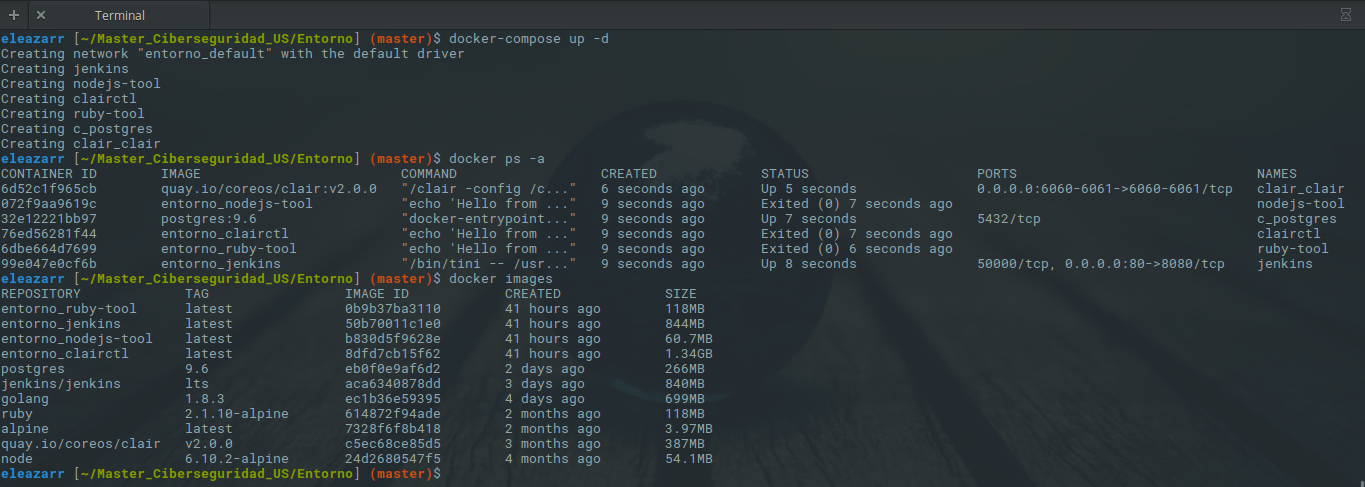
\includegraphics[width=1.0\linewidth]
	{desarrollo/figuras/docker-compose-up.png}
	\caption{Depliegue del entorno con Docker Compose}
	\label{compose}
\end{figure}

\subsection{Probando los componentes desplegados}

Ahora que todos los sistemas están funcionando en el sistema de contenedores es momento de comprobar que la configuración proporcionada es la correcta y que el comportamiento es el esperado. Para ello, y antes de automatizar las tareas con la ayuda de Jenkins, se van a realizar desde el interfaz de comandos las instrucciones necesarias que confirmen que los análisis se están llevando a cabo sin problema por parte de las herramientas de análisis.

El \autoref{prg04-05} muestra la ayuda aportada por el comando "docker exec", que será la utilidad proporcionada por Docker para la ejecución de instrucciones en el interior de los contenedores que se encuentran en ejecución en el entorno (Jenkins, clair\_clair y c\_postgres).

\begin{lstlisting}[language=,caption={Comando de ayuda de docker exec}, breaklines=true, label=prg04-05]
$ docker exec --help

Usage:	docker exec [OPTIONS] CONTAINER COMMAND [ARG...]

Run a command in a running container

Options:
	-d, --detach            Detached mode: run command in the background
	--detach-keys string   	Override the key sequence for detaching a container
	-e, --env list          Set environment variables
	--help                 	Print usage
	-i, --interactive       Keep STDIN open even if not attached
	--privileged           	Give extended privileges to the command
	-t, --tty               Allocate a pseudo-TTY
	-u, --user string       Username or UID (format: <name|uid>[:<group|gid>])
\end{lstlisting}

Para las imágenes de contenedores que no estén en ejecución Docker incluye la utilidad "docker run", con multitud de opciones y argumentos que se adaptan a las ejecuciones más variadas que puedan requerir las imágenes del sistema. El \autoref{prg04-05} ejemplifica el uso de la instrucción que será necesario llevar a cabo en el entorno actual presentado.

\begin{lstlisting}[language=,caption={Comando de ayuda de docker exec}, breaklines=true, label=prg04-06]
$ docker run --help

Usage:	docker run [OPTIONS] IMAGE [COMMAND] [ARG...]

...

$ sudo docker run --rm -t -i -v  ruta_local:ruta_contenedor imagen:tag /bin/bash
root@394bb66c4df0:/home/contenedor# pwd
/home/contenedor
\end{lstlisting}

Donde:

\begin{itemize}
	\item \textit{--rm} indica al demonio de Docker que una vez se termine de trabajar en el contenedor creado, este debe ser eliminado del sistema.
	\item \textit{-t -i} sirve para especificar que se va a abrir un terminal (-t) interactivo (-i) con el contenedor.
	\item \textit{-v} irá continuado por el volumen que se va a montar en el interior del contenedor de Docker.
	\item \textit{imagen:tag} será la imagen utilizada para crear el contenedor.
	\item \textit{/bin/bash} va a ser la instrucción ejecutada una vez creado el contenedor. Este comando va a devolver al usuario un terminal bash interactivo desde el interior del contenedor, donde poder ejecutar las instrucciones necesarias.
\end{itemize}

Conocidos estos comando y utilidades será posible comprobar la funcionalidad del sistema montado.

\subsubsection{Bundler Audit}

El \autoref{prg04-07} muestra los pasos a seguir para comprobar que Bundler Audit funciona correctamente desde el contenedor de Docker.

\begin{lstlisting}[language=,caption={Probando bundle-audit desde el contenedor}, breaklines=true, label=prg04-07]
eleazarr [~/Master_Ciberseguridad_US/Entorno] (master)$ docker run --rm -ti entorno_ruby-tool:latest sh

/ # curl https://raw.githubusercontent.com/EleazarWorkshare/gemfile_vulnerable/master/Gemfile.lock -o ./Gemfile.lock -s
/ # curl https://raw.githubusercontent.com/EleazarWorkshare/gemfile_vulnerable/master/Gemfile -o ./Gemfile -s

/ # bundle-audit check
Name: activesupport
Version: 4.1.1
Advisory: CVE-2015-3226
Criticality: Unknown
URL: https://groups.google.com/forum/#!topic/ruby-security-ann/7VlB_pck3hU
Title: XSS Vulnerability in ActiveSupport::JSON.encode
Solution: upgrade to >= 4.2.2, ~> 4.1.11

Name: activesupport
Version: 4.1.1
Advisory: CVE-2015-3227
Criticality: Unknown
URL: https://groups.google.com/forum/#!topic/rubyonrails-security/bahr2JLnxvk
Title: Possible Denial of Service attack in Active Support
Solution: upgrade to >= 4.2.2, ~> 4.1.11, ~> 3.2.22

Vulnerabilities found!

\end{lstlisting}

Analizando la ejecución en detalle:

\begin{enumerate}
	\item Se accede al contenedor que incluye la herramienta Bundle Audit.
	\item Mediante la \gls{API} de GitHub se descarga desde el repositorio que se quiere analizar los ficheros \textit{Gemfile} y \textit{Gemfile.lock} que incluyen las dependencias de la aplicación examinada.
	\item "bundle-audit check" examina los ficheros, descubriendo que existen vulnerabilidades en la versión 4.1.1 de la dependencia \textit{activesupport} contenida en el repositorio.
\end{enumerate}

\subsubsection{NSP}

El funcionamiento de nsp en el terminal de comando es muy similar al de bundler-audit, como demuestra la \autoref{nsp}.


\begin{figure}[htbp]
	\centering
	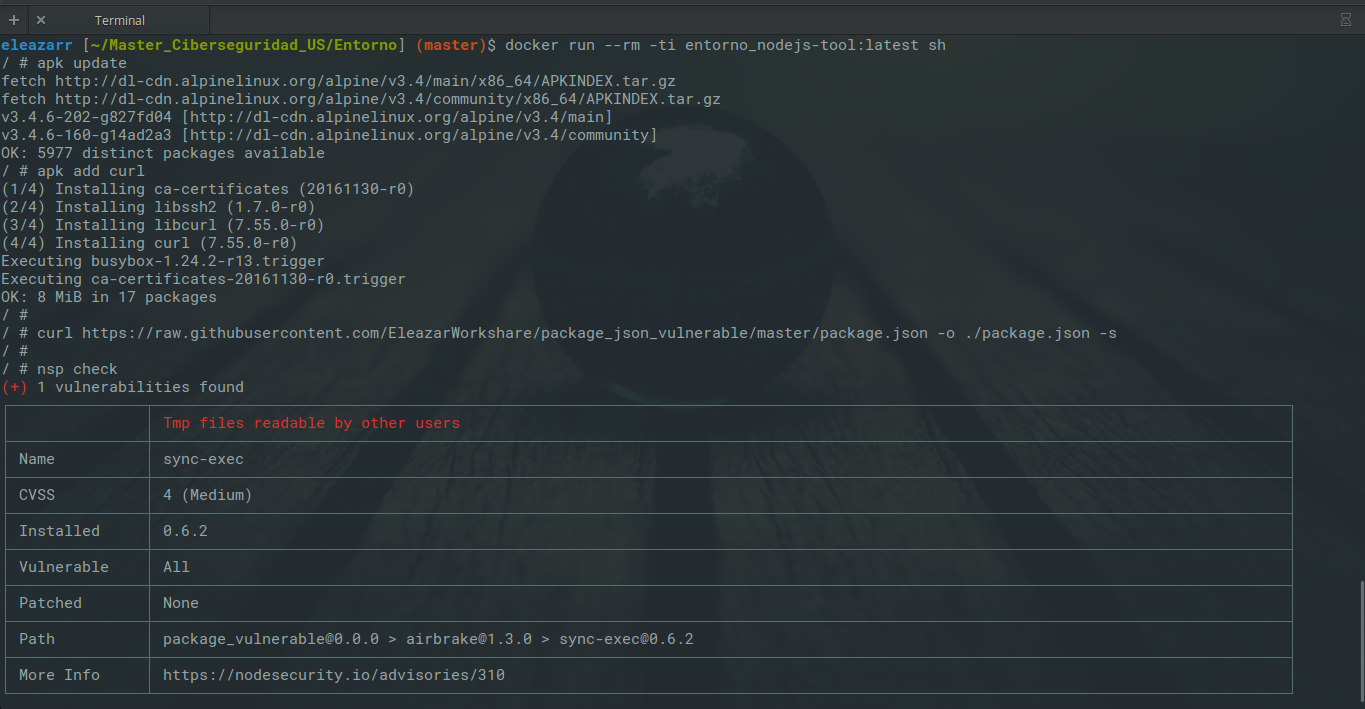
\includegraphics[width=1.0\linewidth]
	{desarrollo/figuras/nsp.png}
	\caption{Comprobando la utilidad nsp}
	\label{nsp}
\end{figure}

\TODO{UN PARRAFO MAS EXPLICANDO LA IMAGEN}

Con lo que queda demostrado que es posible desde el contenedor que ejecuta nsp acceder a la \gls{API} de GitHub, descargar un archivo \textit{package.json} con las dependencias de la aplicación node y realizar un análisis sobre este.

\subsubsection{Clair y Clairctl}

La forma de funcionamiento de Clairctl con Clair es diferente a las vistas para Bundler Audit y NSP, ya que Clairctl requiere de una configuración apropiada que le permita comunicarse con Clair y deberá realizar una serie de pasos para ello:

\begin{enumerate}
	\item Enviará la imagen que se quiere analizar a Clair para que la almacene (push). Dicha imagen podrá encontrarse en la máquina local que contiene a Clairctl o en un repositorio de imágenes de internet (pull).
	\item Clairctl pedirá a Clair que analiza la imagen enviada y le devuelva el resultado de dicho análisis (analyze).
	\item Clairctl generará un informe en formato HTML que podrá ser visualizado en el navegador del usuario.
\end{enumerate}

El proceso comentado se traduce en un mínimo de dos instrucciones de terminal para Clairctl: una para enviar y analizar la imagen en Clair y otra para realizar los informes. El \autoref{prg04-08} muestra el resultado de estas ejecuciones, tomando como ejemplo la propia imagen que contiene a Clairctl.

\begin{lstlisting}[language=,caption={Generando un informe HTML con Clairctl}, breaklines=true, label=prg04-08]
eleazarr [~/Master_Ciberseguridad_US/Entorno] (master)$ docker run --rm -ti -v /home/eleazarr/informe_clairctl:/go/src/github.com/jgsqware/clairctl/reports -v /var/run/docker.sock:/var/run/docker.sock:ro --net entorno_default --link clair_clair:clair -p 57330:57330 entorno_clairctl bash
root@59d0b5391fc6:/go# cd src/github.com/jgsqware/clairctl/
root@59d0b5391fc6:/go/src/github.com/jgsqware/clairctl# clairctl health

Clair: ✔

root@59d0b5391fc6:/go/src/github.com/jgsqware/clairctl# ./clairctl analyze --local entorno_clairctl:latest
2017-09-03 18:03:45.717118 I | config: retrieving interface for local IP
2017-09-03 18:03:45.717535 I | server: Starting Server on 172.20.0.4:57330
2017-09-03 18:03:45.722495 I | config: retrieving interface for local IP
2017-09-03 18:03:45.722730 I | clair: using http://172.20.0.4:57330/local as local url
2017-09-03 18:03:45.722748 I | clair: Pushing Layer 1/9 [b3ddc1248fc3]
2017-09-03 18:03:46.651866 I | clair: Pushing Layer 2/9 [b7f7dd16a445]
2017-09-03 18:03:46.654461 I | clair: Pushing Layer 3/9 [85ac2ce41a64]
2017-09-03 18:03:46.656823 I | clair: Pushing Layer 4/9 [089137f68fc4]
2017-09-03 18:03:46.658893 I | clair: Pushing Layer 5/9 [382f1b17bd70]
2017-09-03 18:03:46.660915 I | clair: Pushing Layer 6/9 [fef71688ca46]
2017-09-03 18:03:46.662980 I | clair: Pushing Layer 7/9 [71e3be3b4746]
2017-09-03 18:03:46.664839 I | clair: Pushing Layer 8/9 [76ceb8887997]
2017-09-03 18:03:46.666559 I | clair: Pushing Layer 9/9 [5ee4b01f03bd]
2017-09-03 18:03:46.668400 I | config: retrieving interface for local IP
2017-09-03 18:03:46.668611 I | clair: using http://172.20.0.4:57330/local as local url
2017-09-03 18:04:03.116083 I | clair: analysing layer [5ee4b01f03bd] 1/9
2017-09-03 18:04:03.143454 I | clair: analysing layer [76ceb8887997] 2/9
2017-09-03 18:04:03.190460 I | clair: analysing layer [71e3be3b4746] 3/9
2017-09-03 18:04:03.212756 I | clair: analysing layer [fef71688ca46] 4/9
2017-09-03 18:04:03.238765 I | clair: analysing layer [382f1b17bd70] 5/9
2017-09-03 18:04:03.285257 I | clair: analysing layer [089137f68fc4] 6/9
2017-09-03 18:04:03.302773 I | clair: analysing layer [85ac2ce41a64] 7/9
2017-09-03 18:04:03.316155 I | clair: analysing layer [b7f7dd16a445] 8/9
2017-09-03 18:04:03.325171 I | clair: analysing layer [b3ddc1248fc3] 9/9

Image: docker.io/entorno_clairctl:latest

Unknown: 15
Negligible: 65
Low: 49
Medium: 83
High: 37
Critical: 0
Defcon1: 0
root@59d0b5391fc6:/go/src/github.com/jgsqware/clairctl# ./clairctl report --local entorno_clairctl:latest                  

HTML report at ./reports/html/analysis-entorno_clairctl-latest.html
\end{lstlisting}

La \autoref{informe} muestra el resultado generado por Clairctl en el análisis de su propia imagen de Docker, confirmando que el sistema al completo se encuentra en perfecto estado de funcionamiento.

\begin{figure}[htbp]
	\centering
	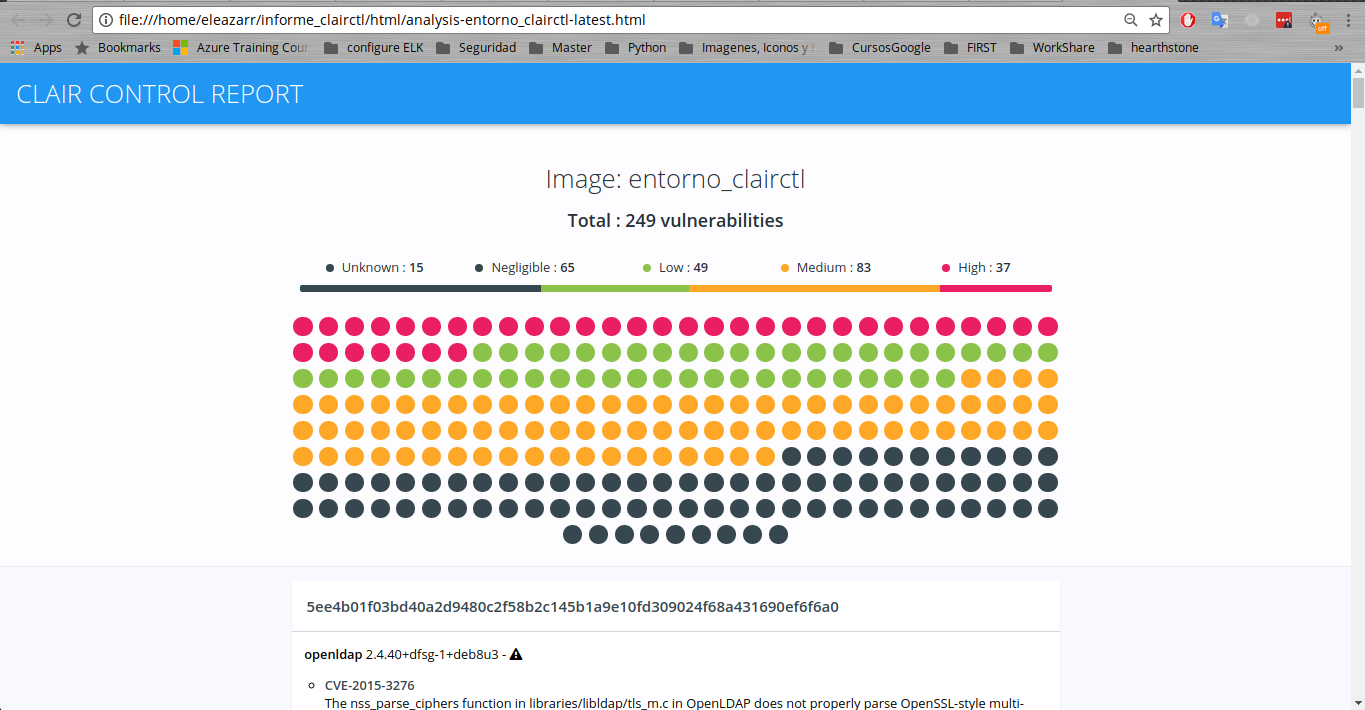
\includegraphics[width=1.0\linewidth]
	{desarrollo/figuras/informe_clairctl.png}
	\caption{Inorme generado por Clairctl}
	\label{informe}
\end{figure}

\subsubsection{Jenkins CI}

Para concluir el apartado se va a confirmar que existe el acceso apropiado al panel de trabajo de Jenkins, así como que se dispone de los plugins necesarios instalados para poder automatizar los trabajos de Jenkins, más conocidos por su traducción al inglés Jenkins Jobs.

En primer lugar, la \autoref{jenkins_01} muestra el mensaje de bienvenida que el usuario encontrará la primera vez que accede a la URL de la aplicación, solicitando un código oculto en el sistema de archivos de la misma. La \autoref{jenkins_02} muestra el acceso al código necesario para comenzar a crear el primer usuario de Jenkins.


\begin{figure}[htbp]
	\centering
	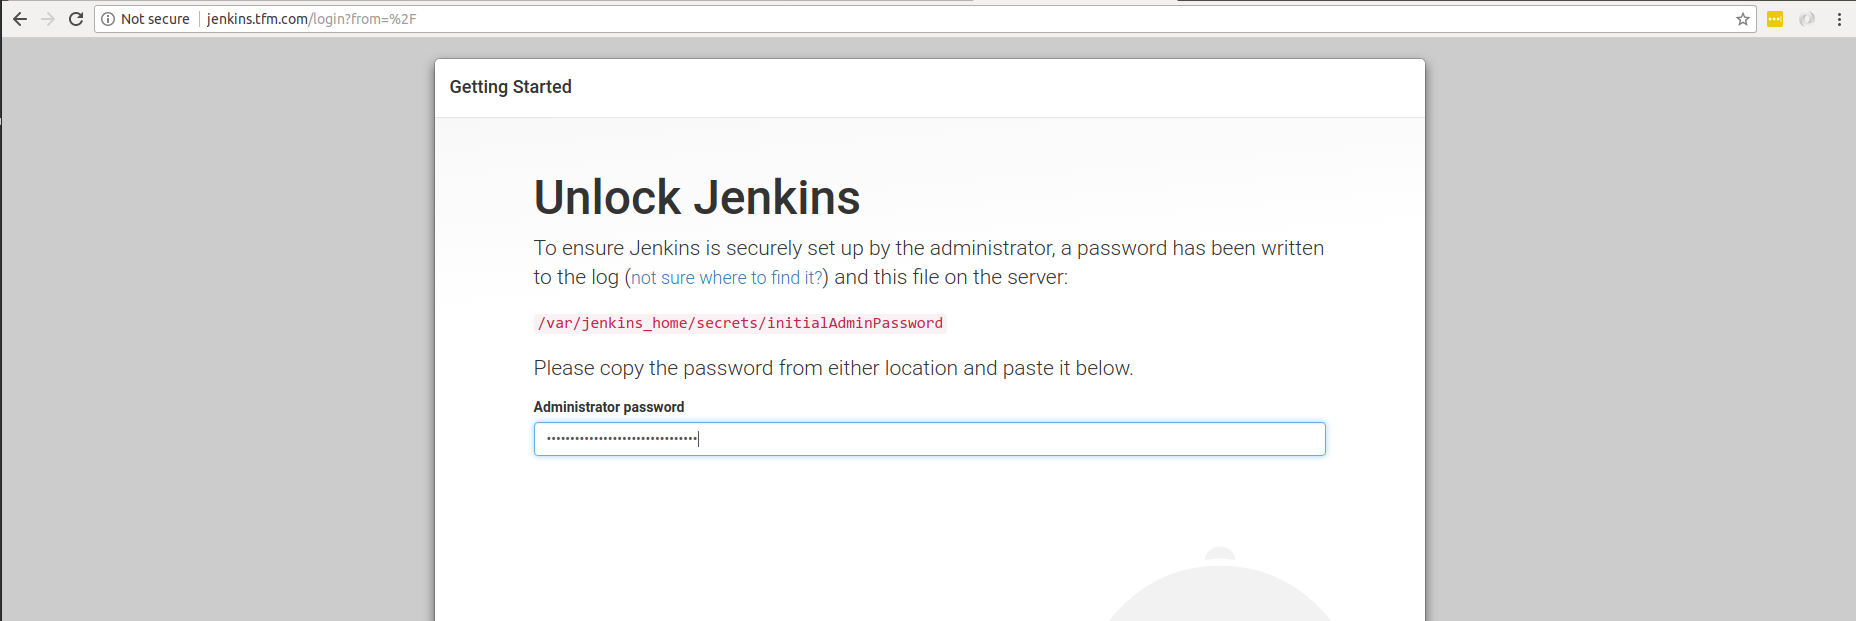
\includegraphics[width=1.0\linewidth]
	{desarrollo/figuras/jenkins_01.png}
	\caption{Bienvenida a la aplicación}
	\label{jenkins_01}
\end{figure}


\begin{figure}[htbp]
	\centering
	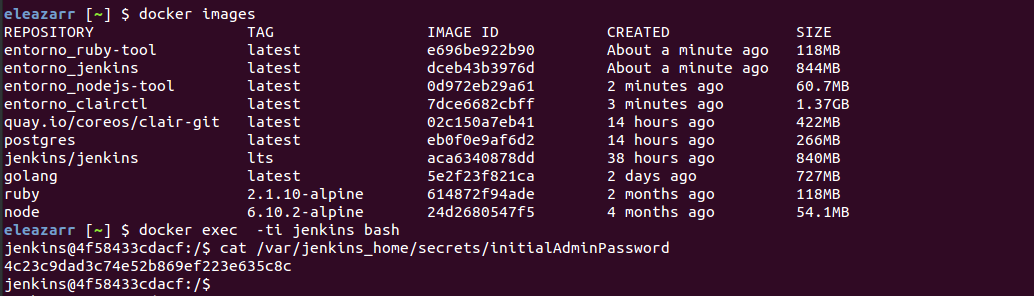
\includegraphics[width=1.0\linewidth]
	{desarrollo/figuras/jenkins_02.png}
	\caption{Encontrando el código oculto}
	\label{jenkins_02}
\end{figure}

Una vez superado la pantalla de bienvenida a la aplicación, se podrá decidir los plugins que serán instalados al inicio (\autoref{jenkins_03}) y comenzará el proceso de instalación inicial de plugins (\autoref{jenkins_04}).


\begin{figure}[htbp]
	\centering
	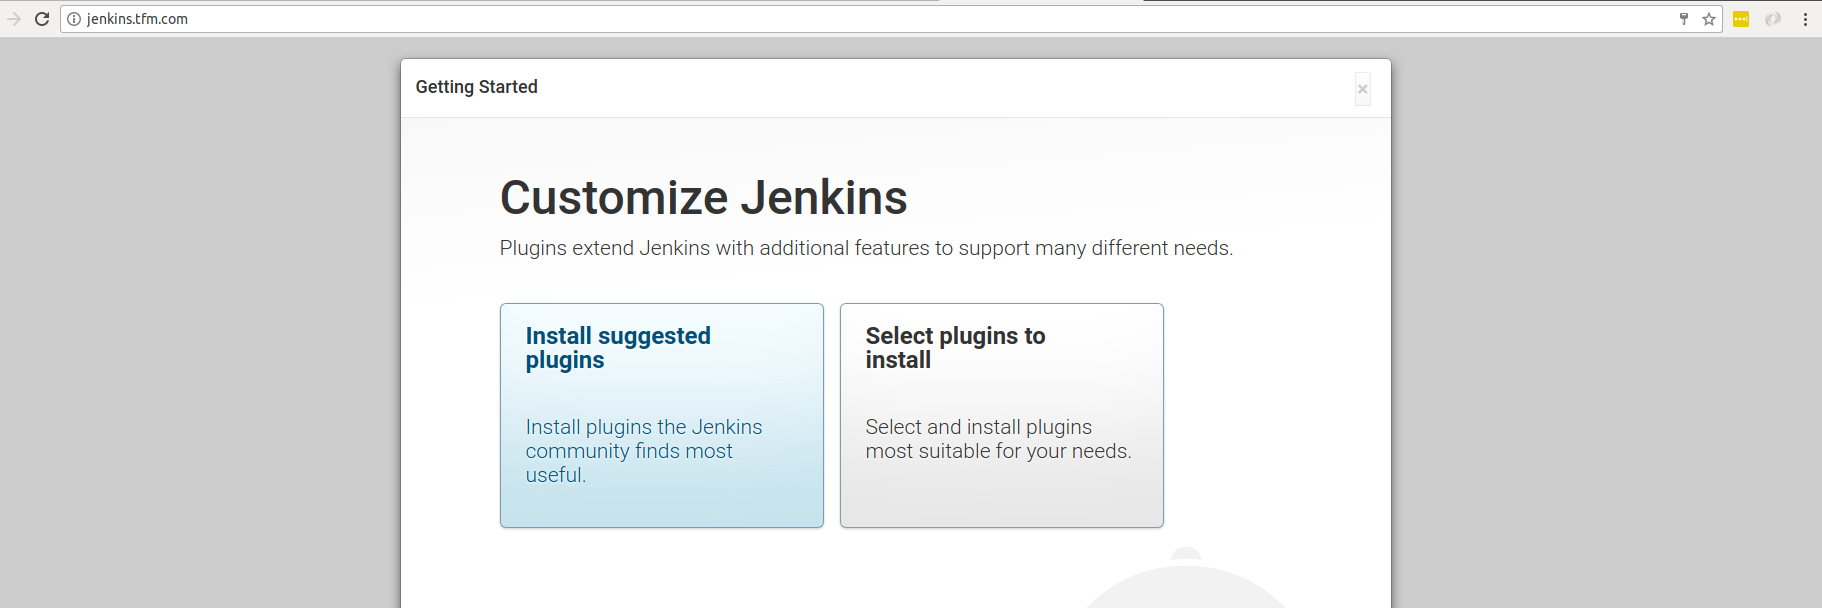
\includegraphics[width=1.0\linewidth]
	{desarrollo/figuras/jenkins_03.png}
	\caption{Instalando plugins recomendados}
	\label{jenkins_03}
\end{figure}

\begin{figure}[htbp]
	\centering
	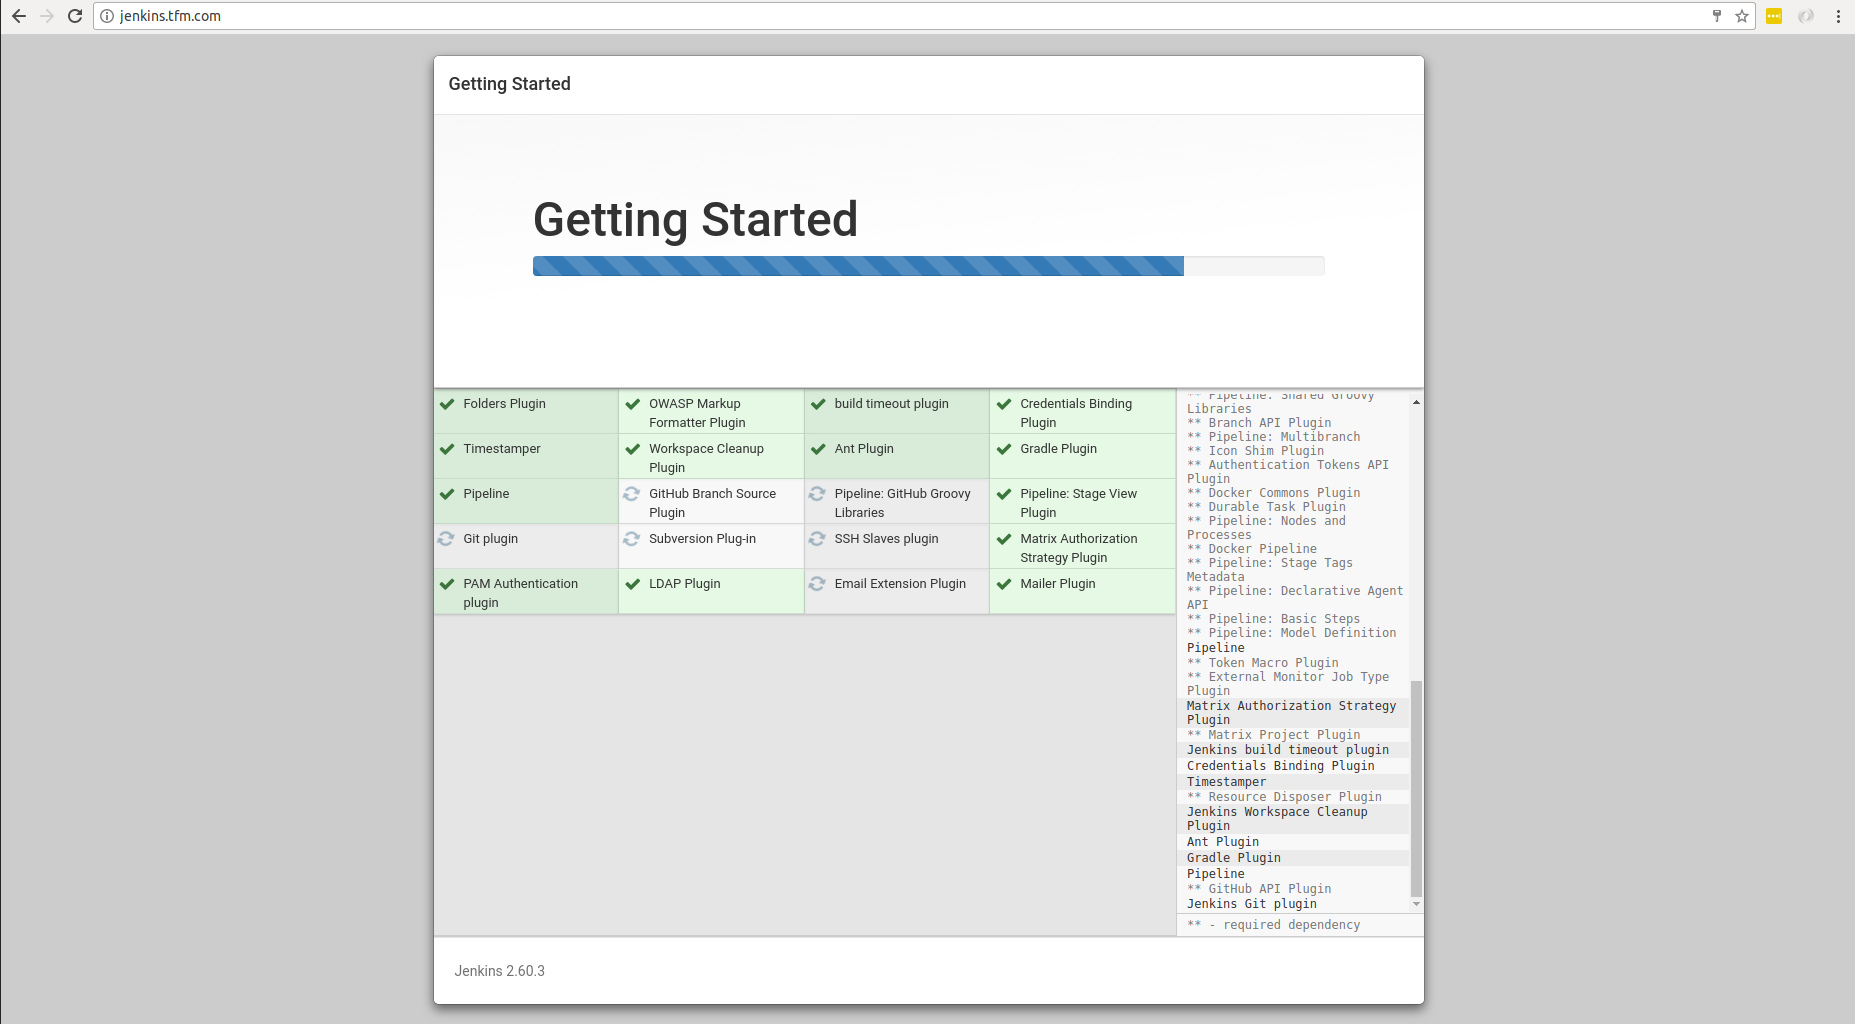
\includegraphics[width=1.0\linewidth]
	{desarrollo/figuras/jenkins_04.png}
	\caption{Proceso de instalación de plugins}
	\label{jenkins_04}
\end{figure}

El último paso de la preparación inicial será crear al primero de los usuarios administrador de la aplicación, la \autoref{jenkins_05} muestra al usuario creado.

\begin{figure}[htbp]
	\centering
	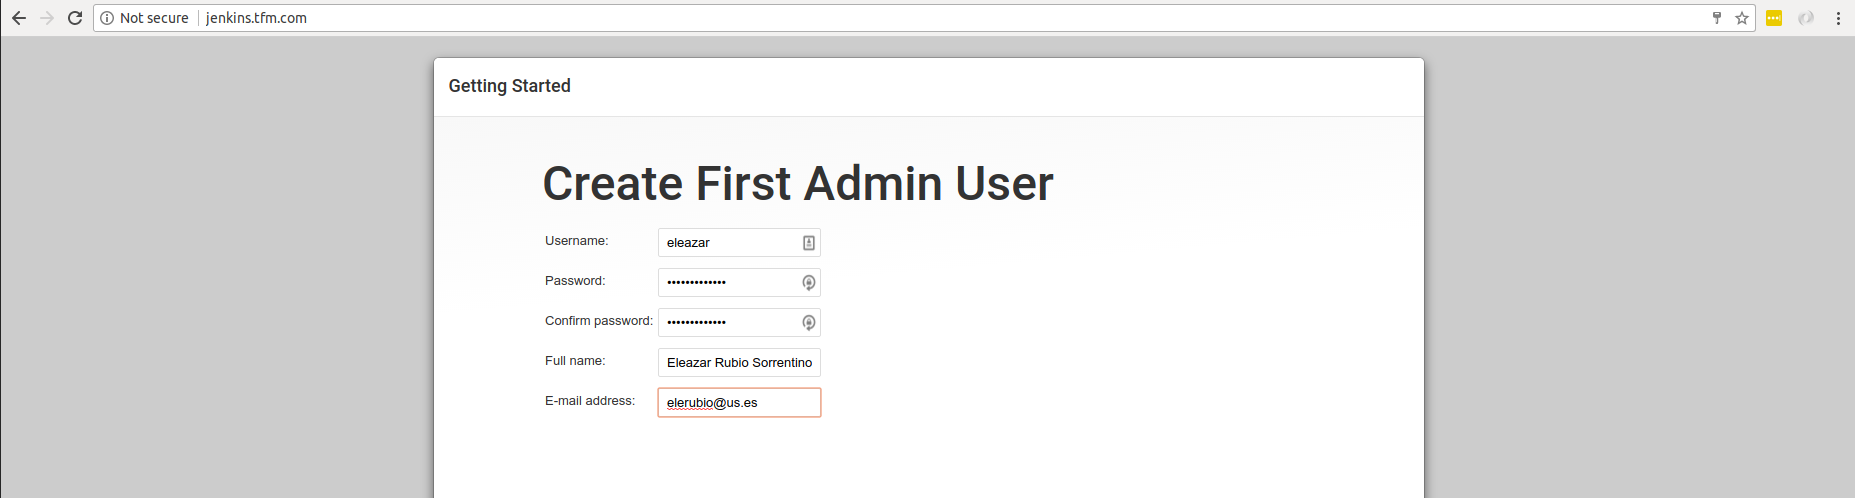
\includegraphics[width=1.0\linewidth]
	{desarrollo/figuras/jenkins_05.png}
	\caption{Creando el primer usuario administrador}
	\label{jenkins_05}
\end{figure}

Con esto la aplicación queda configurada y puede comenzar a usarse (\autoref{jenkins_06}).

\begin{figure}[htbp]
	\centering
	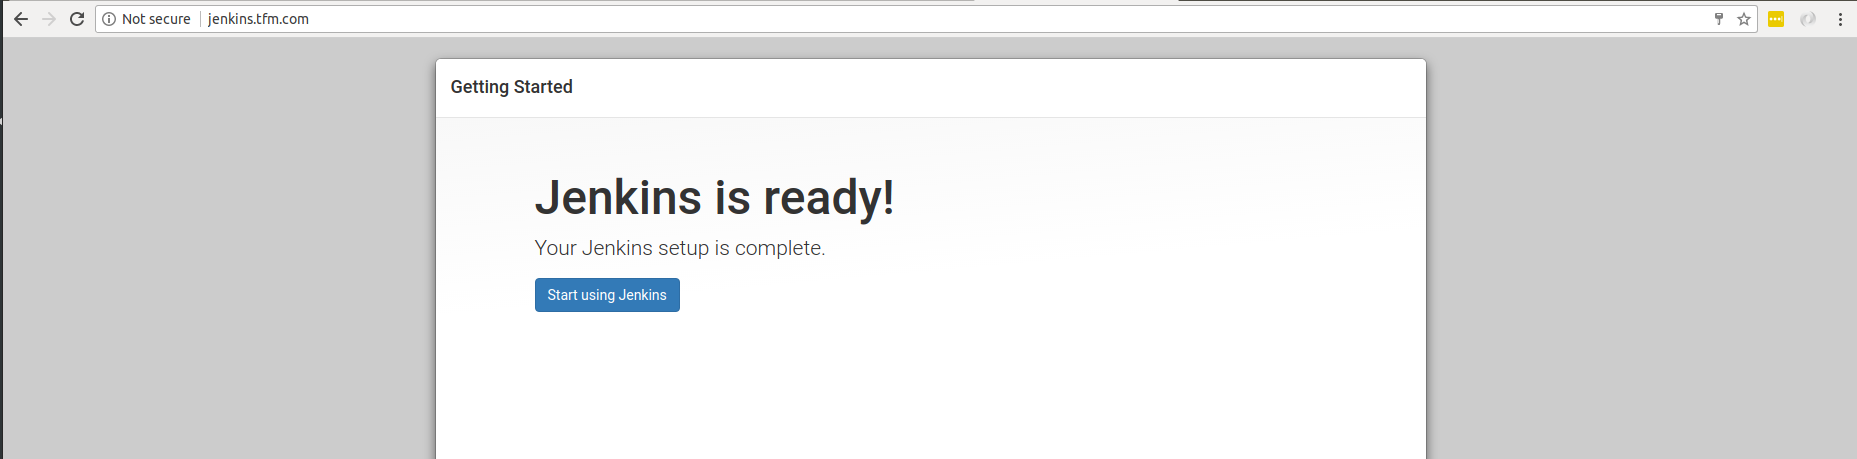
\includegraphics[width=1.0\linewidth]
	{desarrollo/figuras/jenkins_06.png}
	\caption{!Jenkins está listo!}
	\label{jenkins_06}
\end{figure}

Una vez Jenkins está configurado, lo primero que se deberá hacer para poder llevar a cabo el objetivo del presente \gls{TFM} será instalar el plugin \textit{HTML\_publisher}, puesto que será utilizando este como se crearán los informes HTML resultado de la ejecución de cada análisis estático. Las figuras \ref{jenkins_07} y \ref{jenkins_08} muestran las pantallas recorridas.

\begin{figure}[htbp]
	\centering
	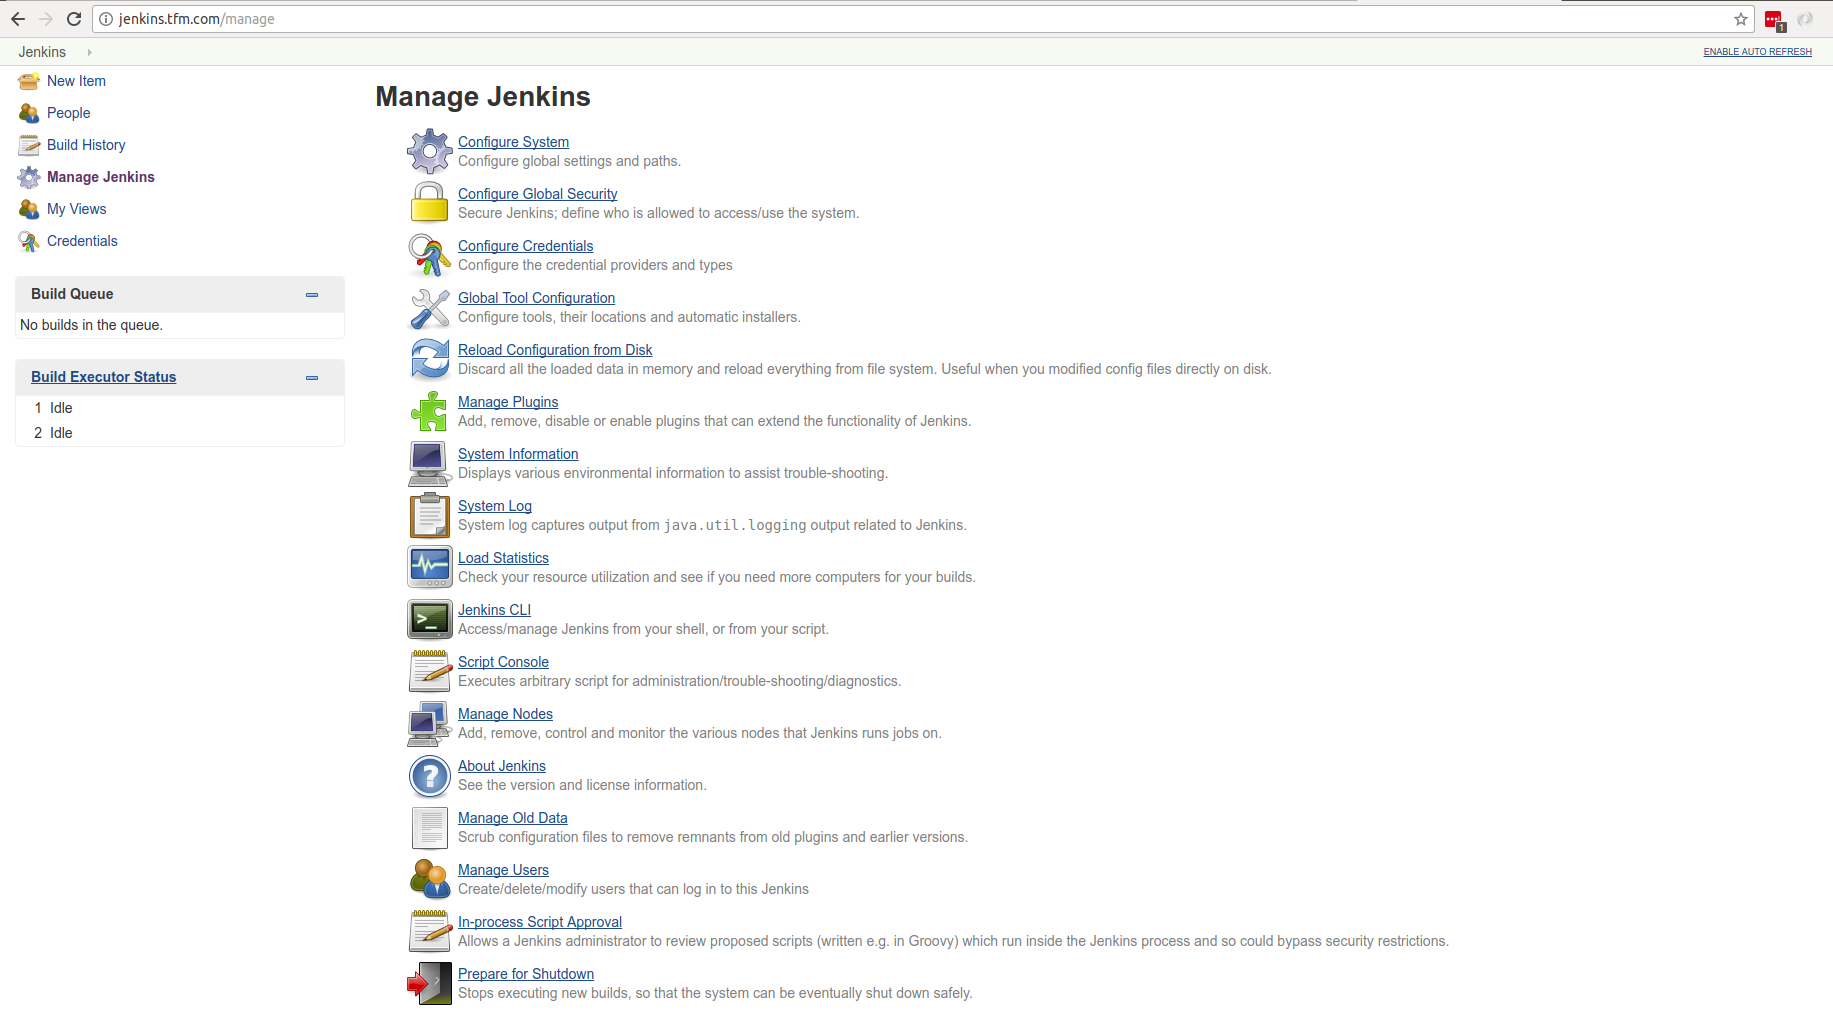
\includegraphics[width=1.0\linewidth]
	{desarrollo/figuras/jenkins_07.png}
	\caption{Manage Jenkins -> Manage Plugins}
	\label{jenkins_07}
\end{figure}

\begin{figure}[htbp]
	\centering
	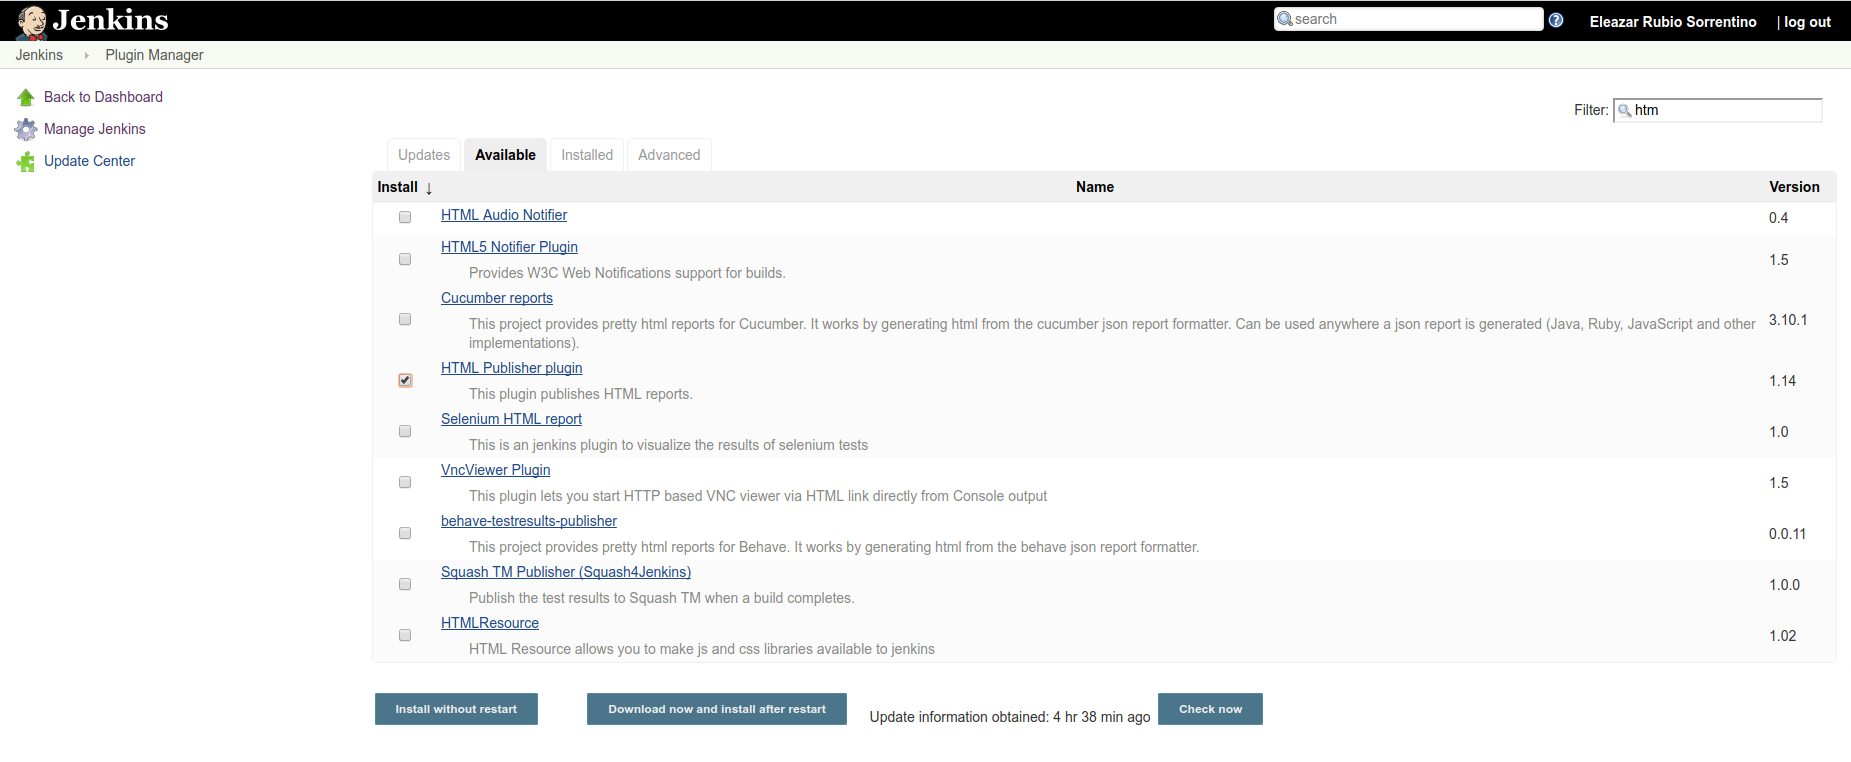
\includegraphics[width=1.0\linewidth]
	{desarrollo/figuras/jenkins_08.png}
	\caption{Instalando HTML\_publisher}
	\label{jenkins_08}
\end{figure}

Tras aplicar la instalación del plugin, y como muestra la \autoref{jenkins_09}, Jenkins se reiniciará, devolviendo al usuario al panel principal (\autoref{jenkins_10}) de la aplicación, con el entorno completamente configurado para comenzar a añadir los trabajos de Jenkins que automatizarán el proceso de análisis.

\begin{figure}[htbp]
	\centering
	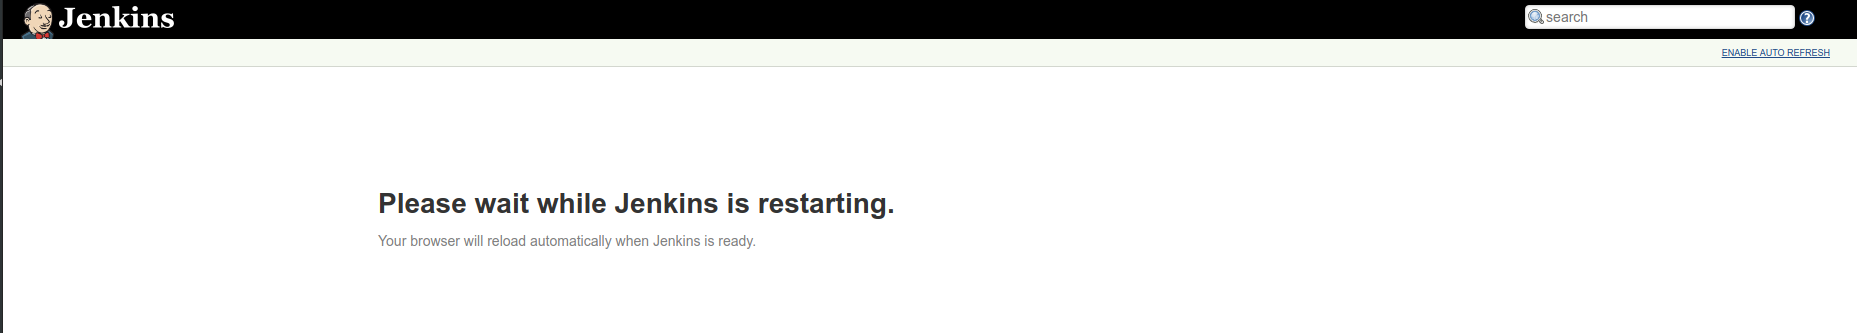
\includegraphics[width=1.0\linewidth]
	{desarrollo/figuras/jenkins_09.png}
	\caption{Reiniciando la aplicación tras la instalación del plugin}
	\label{jenkins_09}
\end{figure}

\begin{figure}[htbp]
	\centering
	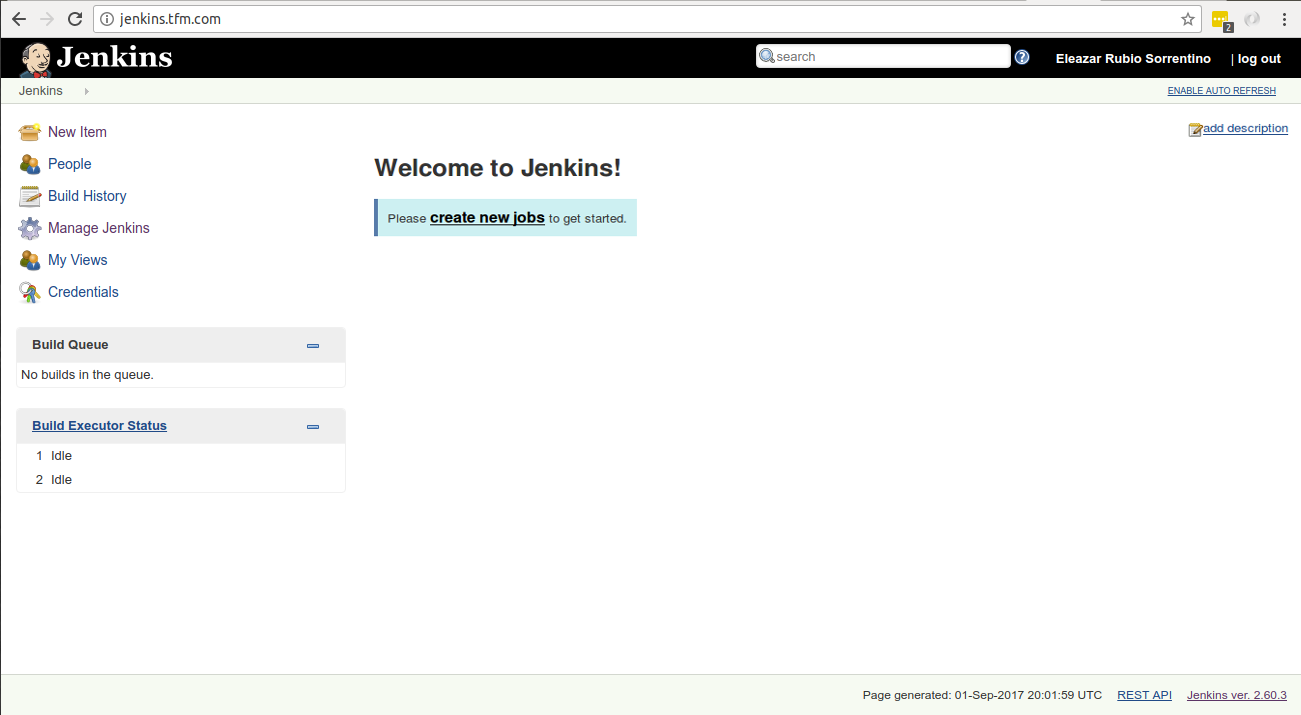
\includegraphics[width=1.0\linewidth]
	{desarrollo/figuras/jenkins_10.png}
	\caption{Pantalla de inicio de Jenkins \gls{CI}}
	\label{jenkins_10}
\end{figure}

\section{Trabajando con Jenkins}\label{trabajando_jenkins}

En la sección actual se va a utilizar el contenido empleado en los apartados de la \autoref{preparacion} para mostrar al lector la creación de tareas o trabajos en la plataforma de \gls{IC} Jenkins, con el fin de automatizar el proceso de análisis de las dependencias de código de aplicaciones escritas mediante los lenguajes de programación Ruby y Node.js, asi como el análisis de las posibles vulnerabilidades que pudieran mantener los contenedores de Docker utilizados por la compañía.

\subsection{Análisis de imágenes Docker}

\subsection{Análisis de dependencias Ruby}

\subsection{Análisis de de dependencias Node.js}

\section{Evaluación de la solución}

ALGUNAS EJECUCIONES QUE MUESTREN VULNERABILIDADES Y SOLUCIONAR ALGUNA.

\section{Resultados obtenidos}

CIERRE DEL APARTADO

\endinput
